In 1999, Frédéric Voisin initiates a project called \textsl{Neuromuse}\footnote{\href{http://www.fredvoisin.com/spip.php?article7}{\texttt{\scriptsize http://www.fredvoisin.com/spip.php?article7}}}\footnote{\href{http://www.neuromuse.org/}{\texttt{\scriptsize http://www.neuromuse.org/}}} based on the artificial neural network, in order to experiment an `organic' interactivity human/machine in a musical context and in real time.

\bigskip

\textsl{Neuromuse3}\footnote{\href{https://github.com/yannics/N3}{\texttt{\scriptsize https://github.com/yannics/N3}}} aims to develop this idea in a holistic way in term of cliques and \textit{tournois}, inspired by the reading of the book \textit{Petite mathématique du cerveau} \citep{bg1} (and also \citep{bg2}, \citep{bg3} and \citep{bg4}).
Then, the object is to create an associative memory able to store and to retrace learned musical sequences, and to create original sequences from this `network of memory' algorithmically.

The real time interactivity consists to a supervised learning according to previous learning as an acquis and a circumstantial recalling process(es) in terms of interactivity and interrelationship.

\bigskip

The formalisation of \textsl{Neuromuse3} is reduced in three main classes defined as NEURON, MLT (superclass of SOM, itself superclass of RNA) and AREA.

The overall mode of operation of \textsl{Neuromuse3} is to stimulate one or more SOM in order to activate a region defined by the AREA and to interpret the response, which can be summarised by the diagram on figure \ref{fig:io}.

\begin{figure}[htbp]
\begin{center}
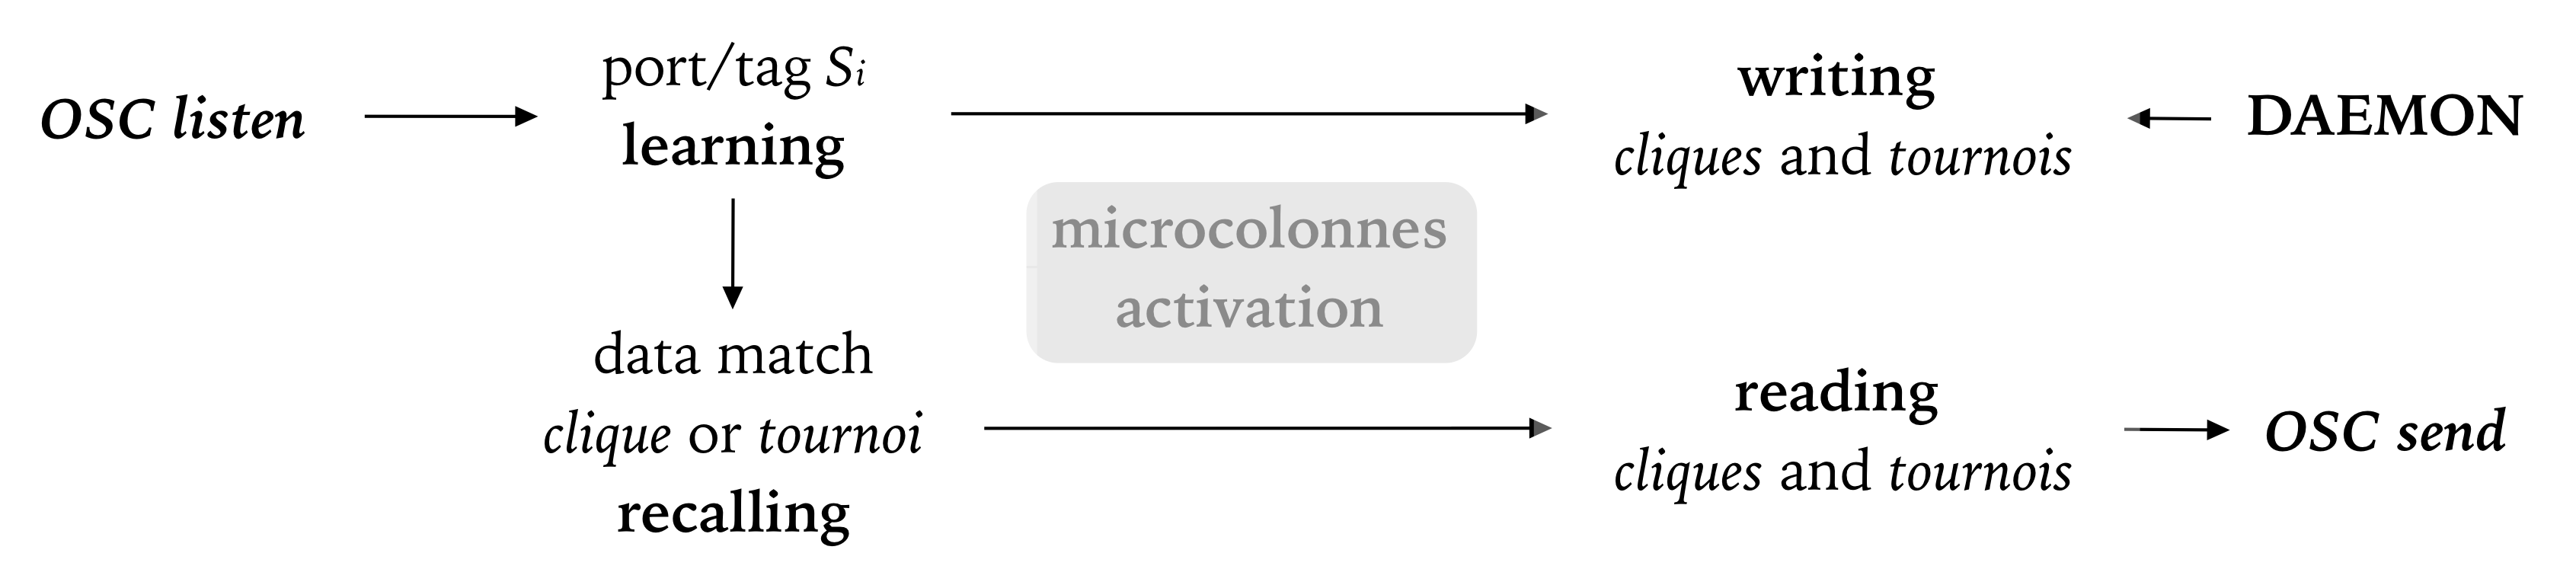
\includegraphics[width=\columnwidth]{2301}
\caption{Synoptic diagram of the I/O management. 
}
\label{fig:io}
\end{center}
\end{figure}

The AREA network can also be interpreted as it is with its inner connectionist structure.